\documentclass[fontsize=11pt]{article}
\usepackage[utf8]{inputenc}
\usepackage[margin=0.75in]{geometry}
\usepackage[utf8]{inputenc}
\usepackage[margin=0.75in]{geometry}
\usepackage{amsmath}
\usepackage{amssymb}
\usepackage{amsthm}
\usepackage{minted}
\usepackage{float}
%%% used to create the bibliography:
\usepackage[lite]{amsrefs}

%%% The following command defines the standard names for all of the
%%% special symbols in the AMSfonts package, listed in
%%% http://www.ctan.org/tex-archive/info/symbols/math/symbols.pdf
\usepackage{amssymb}

%%% The following commands allow you to use \Xy-pic to draw
%%% commutative diagrams.  (You can omit the second line if you want
%%% the default style of the nodes to be \textstyle.)
\usepackage[all,cmtip]{xy}
\let\objectstyle=\displaystyle

%%% If you'll be importing any graphics, uncomment the following
%%% line.  (Note: The spelling is correct; the package graphicx.sty is
%%% the updated version of the older graphics.sty.)
% \usepackage{graphicx}



%%% This part of the file (after the \documentclass command,
%%% but before the \begin{document}) is called the ``preamble''.
%%% This is where we put our macro definitions.

%%% Comment out (or delete) any of these that you don't want to use.
\newcommand{\tensor}{\otimes}
\newcommand{\homotopic}{\simeq}
\newcommand{\homeq}{\cong}
\newcommand{\iso}{\approx}

\DeclareMathOperator{\ho}{Ho}
\DeclareMathOperator*{\colim}{colim}

\newcommand{\R}{\mathbb{R}}
\newcommand{\C}{\mathbb{C}}
\newcommand{\Z}{\mathbb{Z}}

\newcommand{\M}{\mathcal{M}}
\newcommand{\W}{\mathcal{W}}

\newcommand{\itilde}{\tilde{\imath}}
\newcommand{\jtilde}{\tilde{\jmath}}
\newcommand{\ihat}{\hat{\imath}}
\newcommand{\jhat}{\hat{\jmath}}



%%%-------------------------------------------------------------------
%%%-------------------------------------------------------------------
%%% The Theorem environments:
%%%
%%%
%%% The following commands set it up so that:
%%% 
%%% All Theorems, Corollaries, Lemmas, Propositions, Definitions,
%%% Remarks, Examples, Notations, and Terminologies  will be numbered
%%% in a single sequence, and the numbering will be within each
%%% section.  Displayed equations will be numbered in the same
%%% sequence. 
%%% 
%%% 
%%% Theorems, Propositions, Lemmas, and Corollaries will have the most
%%% formal typesetting.
%%% 
%%% Definitions will have the next level of formality.
%%% 
%%% Remarks, Examples, Notations, and Terminologies will be the least
%%% formal.
%%% 
%%% Theorem:
%%% \begin{thm}
%%% 
%%% \end{thm}
%%% 
%%% Corollary:
%%% \begin{cor}
%%% 
%%% \end{cor}
%%% 
%%% Lemma:
%%% \begin{lem}
%%% 
%%% \end{lem}
%%% 
%%% Proposition:
%%% \begin{prop}
%%% 
%%% \end{prop}
%%% 
%%% Definition:
%%% \begin{defn}
%%% 
%%% \end{defn}
%%% 
%%% Remark:
%%% \begin{rem}
%%% 
%%% \end{rem}
%%% 
%%% Example:
%%% \begin{ex}
%%% 
%%% \end{ex}
%%% 
%%% Notation:
%%% \begin{notation}
%%% 
%%% \end{notation}
%%% 
%%% Terminology:
%%% \begin{terminology}
%%% 
%%% \end{terminology}
%%% 
%%%       Theorem environments

% The following causes equations to be numbered within sections
\numberwithin{equation}{section}

% We'll use the equation counter for all our theorem environments, so
% that everything will be numbered in the same sequence.

%       Theorem environments

\theoremstyle{plain} %% This is the default, anyway
\newtheorem{thm}[equation]{Theorem}
\newtheorem{cor}[equation]{Corollary}
\newtheorem{lem}[equation]{Lemma}
\newtheorem{prop}[equation]{Proposition}

\theoremstyle{definition}
\newtheorem{defn}[equation]{Definition}

\theoremstyle{remark}
\newtheorem{rem}[equation]{Remark}
\newtheorem{ex}[equation]{Example}
\newtheorem{notation}[equation]{Notation}
\newtheorem{terminology}[equation]{Terminology}


\usepackage{graphicx}
\usepackage{fancyref}
\usepackage{tikz,pgfplots}


%%%-------------------------------------------------------------------
%%%-------------------------------------------------------------------
%%%-------------------------------------------------------------------
%%%-------------------------------------------------------------------
%%%-------------------------------------------------------------------
%%%-------------------------------------------------------------------
%%%-------------------------------------------------------------------
\pgfplotsset{compat=1.18}

\title{CSC111H Project Report: Harmonify}
\author{Mert Rassa, Salih Atamert Cam, Ece Avşar}
\date{Sunday, March 30, 2025}

\begin{document}
\maketitle

\section*{1 Introduction}
  $\qquad $From ancient times to present, humans have always yearned for social interaction. Whether for education, friendship, or relationships, we are inherently social beings. Throughout the years, this interaction has taken on all sorts of form. While in the past, people could only interact with others from far away through letters, nowadays you can interact with someone thousands of kilometers away, with only one simple click. Through communicative online platforms, people can become friends really easily. 
  Music is one of the other main ways to connect people. It is a strong sense that helps people have fun and communicate even without speaking! 

  So, what about a program that combines these concepts? 
  
  Meet Harmonify!
  \\

  If you are a "musicophile" and looking to connect with others who share your taste in music, and you are also tired of listening to the same songs on repeat, then "Harmonify" is the perfect place to find your underlying "rhythm" with music and other people! With our project “Harmonify”, you can expand your music taste and meet with people that have your same music taste! Inspired by Spotify, which is a digital music platform that gives users access to many different songs from different genres created by inspiring artists all over the world, Harmonify makes this platform more human-interactive by recommending different types of songs to a user depending on their choice of song duration, genre, and their favorite songs. Our project also includes matching / suggesting the user to other users who are most interested in similar songs. By integrating a user-recommendation tool in our project, our project aims to connect people in terms of their similar music interests and create more connections, and aims to answer the question: \textbf{Based on preferred genre, top 5 favorite songs and preferred song duration, how can we recommend new songs and new friends to a user?}
\section*{2 Data sets}

$\qquad$This project uses the Abstract Data Type (ADT) Graph. The graph we implemented has additional features that separates it from the Graph structure we have covered in class, which will be mentioned more in depth in section \textbf{3}. In this project, we have used a graph type also known as "Knowledge Graphs". This graph uses two datasets consisting of certain variables for different observations. Two sample observations for a song and a certain user can be found below: Table~\ref{tab:table1}, Table~\ref{tab:table2}. Table 2 is extracted from: https://www.kaggle.com/datasets/thedevastator/spotify-tracks-genre-dataset 
\\
\begin{table} [h!]
    \centering
    \begin{tabular}{|c|c|c|c|c|}
        \hline
        \textbf{username} & \textbf{name} & \textbf{age} & \textbf{province} & \textbf{song\_id} \\ \hline
        GalaxyDestroyer & Ece & 19 & Toronto & 1 \\ \hline
        GalaxyDestroyer & Ece & 19 & Toronto & 2 \\ \hline
        
    \end{tabular}
    \caption{A sample from user dataset}
    \label{tab:table1}
\end{table}
\\
\begin{table}[h!]
    \centering
    \begin{tabular}{|c|c|c|c|c|}
        \hline
        \textbf{track\_id} & \textbf{track\_name} & \textbf{artists} & \textbf{duration\_ms} & \textbf{track\_genre} \\ \hline
        1 & Unholy (feat. Kim Petras) & Sam Smith;Kim Petras & 156943 & dance \\ \hline
    \end{tabular}
    \caption{A sample from songs dataset}
    \label{tab:table2}
\end{table}
\\

\section*{2.1 Data Wrangling/ Obtaining:}
\textbf{Song Dataset}
\\

The dataset obtained from kaggle included many different variables regarding the songs that were not required for conducting the project, such as "energy", "instrumentalness" and "key". Therefore, we have filtered our dataset using the \textbf{pandas} library, where functions such as DataFrame.drop() and DataFrame.groupby() were used to sort the data and extract the cruical information. 

The dataset also consisted of almost 90,000 songs. Hence, using this whole dataset would increase the runtime complexity and make it more difficult for finding users to match with the input user due to less probability. When the number of songs increases, the possibility of compared users having the common song decreases thus they match with less songs with a much lower similarity score. There were also songs included in our dataset that were not really known. To overcome these problems, the dataset was ranked by "popularity" column that was included in the original dataset, and a subset of our original data with 200 songs were extracted through this code: 

\begin{minted}[frame=single, fontsize=\small]{python}
df = pd.read_csv('all_songs.csv')

# Remove duplicates (keep the first occurrence)
df = df.drop_duplicates()
df_sorted = df.groupby('track_name', sort=False).first().reset_index()

# Sort by 'popularity' in descending order and keep the top 200
df_sorted = df_sorted.sort_values(by='popularity', ascending=False).head(200)

# Drop unnecessary columns from the sorted dataframe
df_sorted = df_sorted.drop(
    columns=['track_id', 'album_name', 'explicit','danceability', 'popularity', 
            'energy', 'time_signature', 'tempo', 'valence','liveness', 'instrumentalness', 'acousticness', 
            'speechiness', 'mode', 'key', 'loudness'],
    errors='ignore'  # Ignore if any column is missing
)

if 'Unnamed: 0' in df.columns:
    df_sorted = df_sorted.drop('Unnamed: 0', axis=1)


# Save the sorted CSV to a new file
df_sorted.to_csv('songs_by_popularity.csv', index_label='Rank', header=False)

\end{minted}

- To create "track\_id" for each song based on their popularity ranking, we have started the index from 1 and incremented for each row up until 200 to get a cleaner dataset.

- After these filterings, we stored \texttt{df\_sorted} within the csv file: \texttt{songs\_by\_popularity.csv}
\\

\textbf{User Dataset}
\\

$\qquad$Creating our user dataset would have required conducting a survey in which participants provided a chosen username for our program, their name, their ten favorite songs, and their current province of residence. This survey would have needed to run over an extended period to gather sufficient user input. However, due to time constraints on our project, we decided to create a synthetic user dataset by asking ChatGPT. Our prompt to extract this user dataset was as follows:

\textit{Create a user dataset with 200 users in the format: "username, name, age, province in Canada, random number from 1 to 200, and every username should have 10 lines associated with 10 random discrete numbers.} We have also added our \texttt{users\_small.csv} as a reference. 
\\

We then stored our full user dataset within \textbf{user\_data\_all\_100.csv} and \textbf{user\_data\_all\_200.csv}. For the first dataset, we only included up to 100 songs and for the second dataset, we only included 200 songs to see how the probability of our program's song recommendation changes as the song amounts change. We have observed that with 200 dataset, our program gave approximately 2 song matches whereas with the 100 dataset, our program gave approximately 3 song matches with each launch.

The range of songs used within the program can be changed through a minor adjustment within the code below, where the function called is \textbf{compute\_algorithm()} in \textbf{main.py}: 

\begin{minted}[frame=single, fontsize=\small]{python}
visualize_graph(load_review_graph('all_user_data_200_songs.csv', 'songs_by_popularity.csv'))
g = load_review_graph('all_user_data_200_songs.csv', 'songs_by_popularity.csv')

\end{minted}

Here, changing the first parameter of \textbf{load\_review\_graph }from all\_user\_data\_200\_songs.csv to all\_user\_data\_200\_songs.csv will increase the chance of getting more songs in common with the input user and the matched user.
\\

\section*{3 Computational Overview:}
\textbf{3.1 Knowledge Graphs:}
\bigskip

Knowledge Graphs are graphs that show the interconnection between certain entities and their relationship. They consist of an "entities" vertex and each "entities" vertex is connected with a relationship, and the connections of each vertex through similar relationships are studied. Hence, knowledge graphs put the data in context by linking semantic data with entities. 

The graph we have constructed consist of two different kinds of vertices: Song and User. These vertices will be distinguished by their "kind" attribute, which is either "song" or "user". In this context, users can be considered "entities" whereas we will be studying the "relationship" between different entities through a semantic data, which are "songs".

Additionally, the graph we have implemented is called a \textbf{bipartite graph}, where no user vertex is adjacent to the song vertex. Hence, every neighbour of user vertex is song vertex and every neighbour of the song vertex is the user vertex.
\\

\textbf{Vertices:}
\begin{itemize}
\item Song vertices have attributes "item" which is a list that includes [Song's name, Song's artist, Song's duration, Song's genre] and a "neighbours" set that includes adjacent vertices which represent the Users that listen to that song. In the Graph, Songs have numerical IDs as their key to be called from '\_Vertices' private dictionary. In addition, in our music data set, we sorted songs by popularity in descending order and gave them id numbers from 1 to 200. So, the song with the highest popularity score has ID = 1.

\item User vertices have attributes "item" which is a list that includes [User's username, User's name, User's age, User's province] and a "neighbours" set that includes the User's adjacent vertices which represent the songs that users listen to. In the graph, Users have their usernames as key to be called from the "\_Vertices" private dictionary.
\end{itemize}
\textbf{3.2 Computations:}
\\

\textbf{Similarity score:}
Our algorithm takes into consideration our implications and interpretations of compatibility score based on user input, and also takes into account the number of edges they both users share. The explanation of our implementation of the similarity score can be found below:
\\
\begin{minted}[frame=single, fontsize=\small]{python}
"""
Similarity score is calculated by finding;
        - the number of common songs listened by this user and the other user,
        - the number of songs that 1) this user and the other user listens and
        2) matches with this user's favourite genre.
        - the number of songs that 1) this user and the other user listens and
        2) duration of the song matches with this user's preferred duration.

        after calculating these values, we find the similarity_score by
        "number_of_common_songs * 3 + number_of_common_genres * 2 number_of_common_duration * 1" formula
"""
\end{minted}

\textbf{Compatible user:}
We implemented \textbf{compatible\_user\_rec\_songs()} function. This function returns new user's most compatible user, the songs they listen in common, the songs only the most compatible user listen, and their matched similarity score.

\textbf{1.} First we created an empty dictionary for all users in the graph and an empty list for the scores. 
Then, we check every vertex in the graph and if the vertex is the kind "user" and different from our input user, we get the similarity score of the new user and the user that was already in the graph with the \textbf{similarity\_score() }function. We store that in the score variable. 

\textbf{2.} If the score is higher than 0, we check if there is already a key with the value of the score in the dictionary. If there is not, we create a key with the score value and that key maps to the user with that score. If there is, we add the user in the graph to the list that our score key maps to.    

\textbf{3.} After checking every vertex, sort the scores list in ascending order then user the \textbf{.pop()} method to get the highest score. We then use this max score as a key to get the most compatible user from the users dictionary (We extract the index 0 because the program only requires 1 compatible user).

\textbf{4.} So now we have the most compatible user's vertex and we use the item attribute to get the parameters of the compatible user.

\textbf{5.} We then create 3 empty lists as :
recommended\_songs
both\_songs\_you\_listen
songs\_user\_listen

\textbf{6.} Then we put the neighbours of the new user to the songs\_user\_listen,
then we check neighbours of the compatible user, if they are listening a song in common we add the song to the both\_songs\_you\_listen. If not we add song to the recommended\_songs.

\textbf{7.} Finally, we return the most compatible users' information, both\_songs\_you\_listen, recommended\_songs, and the compatibility score.

\bigskip

\textbf{Example Graph:}
\begin{figure}[!ht]
\centering
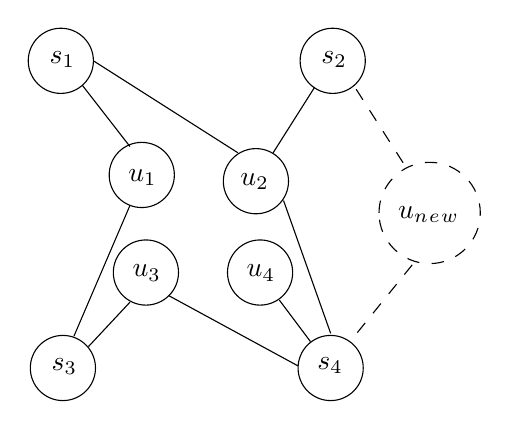
\begin{tikzpicture}[x=0.75pt,y=0.75pt,yscale=-1,xscale=1]
%uncomment if require: \path (0,392); %set diagram left start at 0, and has height of 392

%Shape: Circle [id:dp6243765739969105] 
\draw   (330,184.3) .. controls (330,175.63) and (337.03,168.6) .. (345.7,168.6) .. controls (354.37,168.6) and (361.4,175.63) .. (361.4,184.3) .. controls (361.4,192.97) and (354.37,200) .. (345.7,200) .. controls (337.03,200) and (330,192.97) .. (330,184.3) -- cycle ;
%Shape: Circle [id:dp023554597820756085] 
\draw  [dash pattern={on 4.5pt off 4.5pt}] (403,155.6) .. controls (403,142.12) and (413.92,131.2) .. (427.4,131.2) .. controls (440.88,131.2) and (451.8,142.12) .. (451.8,155.6) .. controls (451.8,169.08) and (440.88,180) .. (427.4,180) .. controls (413.92,180) and (403,169.08) .. (403,155.6) -- cycle ;
%Straight Lines [id:da20480436930836854] 
\draw    (372,95) -- (352,126.6) ;
%Straight Lines [id:da924329529998065] 
\draw    (379.7,213.6) -- (357,149.6) ;
%Straight Lines [id:da7590214990090951] 
\draw    (265.4,82.3) -- (335,126.6) ;
%Shape: Circle [id:dp6392139536325514] 
\draw   (275,184.3) .. controls (275,175.63) and (282.03,168.6) .. (290.7,168.6) .. controls (299.37,168.6) and (306.4,175.63) .. (306.4,184.3) .. controls (306.4,192.97) and (299.37,200) .. (290.7,200) .. controls (282.03,200) and (275,192.97) .. (275,184.3) -- cycle ;
%Shape: Circle [id:dp09959984639549613] 
\draw   (273,137.3) .. controls (273,128.63) and (280.03,121.6) .. (288.7,121.6) .. controls (297.37,121.6) and (304.4,128.63) .. (304.4,137.3) .. controls (304.4,145.97) and (297.37,153) .. (288.7,153) .. controls (280.03,153) and (273,145.97) .. (273,137.3) -- cycle ;
%Shape: Circle [id:dp1342966882871146] 
\draw   (328,140.3) .. controls (328,131.63) and (335.03,124.6) .. (343.7,124.6) .. controls (352.37,124.6) and (359.4,131.63) .. (359.4,140.3) .. controls (359.4,148.97) and (352.37,156) .. (343.7,156) .. controls (335.03,156) and (328,148.97) .. (328,140.3) -- cycle ;
%Straight Lines [id:da4128688701476244] 
\draw  [dash pattern={on 4.5pt off 4.5pt}]  (392,96) -- (416,133.6) ;
%Straight Lines [id:da7438725569856084] 
\draw  [dash pattern={on 4.5pt off 4.5pt}]  (419,180.6) -- (390,216.4) ;
%Straight Lines [id:da6425475579909588] 
\draw    (260,94) -- (283,123.6) ;
%Straight Lines [id:da2897780561922667] 
\draw    (283,152) -- (256,215) ;
%Straight Lines [id:da6936007268806075] 
\draw    (283,198.6) -- (263,220) ;
%Straight Lines [id:da5501307213520161] 
\draw    (302,195.6) -- (364,229.3) ;
%Straight Lines [id:da7500614160388785] 
\draw    (355,197.6) -- (370,217.6) ;
%Shape: Circle [id:dp46846681443933846] 
\draw   (234,82.3) .. controls (234,73.63) and (241.03,66.6) .. (249.7,66.6) .. controls (258.37,66.6) and (265.4,73.63) .. (265.4,82.3) .. controls (265.4,90.97) and (258.37,98) .. (249.7,98) .. controls (241.03,98) and (234,90.97) .. (234,82.3) -- cycle ;
%Shape: Circle [id:dp01636577219505342] 
\draw   (365,82.3) .. controls (365,73.63) and (372.03,66.6) .. (380.7,66.6) .. controls (389.37,66.6) and (396.4,73.63) .. (396.4,82.3) .. controls (396.4,90.97) and (389.37,98) .. (380.7,98) .. controls (372.03,98) and (365,90.97) .. (365,82.3) -- cycle ;
%Shape: Circle [id:dp7276716084774888] 
\draw   (235,230.3) .. controls (235,221.63) and (242.03,214.6) .. (250.7,214.6) .. controls (259.37,214.6) and (266.4,221.63) .. (266.4,230.3) .. controls (266.4,238.97) and (259.37,246) .. (250.7,246) .. controls (242.03,246) and (235,238.97) .. (235,230.3) -- cycle ;
%Shape: Circle [id:dp9312001610423202] 
\draw   (364,230.3) .. controls (364,221.63) and (371.03,214.6) .. (379.7,214.6) .. controls (388.37,214.6) and (395.4,221.63) .. (395.4,230.3) .. controls (395.4,238.97) and (388.37,246) .. (379.7,246) .. controls (371.03,246) and (364,238.97) .. (364,230.3) -- cycle ;

% Text Node
\draw (243,76.4) node [anchor=north west][inner sep=0.75pt]    {$s_{1}$};
% Text Node
\draw (374,76.4) node [anchor=north west][inner sep=0.75pt]    {$s_{2}$};
% Text Node
\draw (244,224.4) node [anchor=north west][inner sep=0.75pt]    {$s_{3}$};
% Text Node
\draw (372,224) node [anchor=north west][inner sep=0.75pt]    {$s_{4}$};
% Text Node
\draw (281,133.4) node [anchor=north west][inner sep=0.75pt]    {$u_{1}$};
% Text Node
\draw (335,135.4) node [anchor=north west][inner sep=0.75pt]    {$u_{2}$};
% Text Node
\draw (283,179.4) node [anchor=north west][inner sep=0.75pt]    {$u_{3}$};
% Text Node
\draw (338,179.4) node [anchor=north west][inner sep=0.75pt]    {$u_{4}$};
% Text Node
\draw (411,151.4) node [anchor=north west][inner sep=0.75pt]    {$u_{n}{}_{e}{}_{w}$};


\end{tikzpicture}
\caption{New user added}
    \label{fig:Example1}
\end{figure}


In Figure \ref{fig:Example1}, we can see that there are already registered users ($u_1$, $u_2$, $u_3$, $u_4$) and the songs they listen to($s_1$, $s_2$, $s_3$, $s_4$). Alongside that, when the new user starts the program, we are going to ask for their username to create a new "temporary" vertex, and top 5 songs they would like to listen to create edges between the songs and the new user. Our example graph in Figure 1 shows that the new registered user $u_{new}$ who started the program and the edges between ($u_{new}$ and $s_2$) and ($u_{new}$ and $s_4$) show that the new user indicated $s_2$ and $s_4$ for their top songs. After making the new additions to the graph, we can see that the new user is listening to the two same songs ($s_2$ and $s_4$) with $u_2$ and the one same song ($s_4$) with $u_4$. By analyzing the genre and duration of the songs, we are going to create a compatibility score for $u_2$ and $u_4$. Finally, we are going to return the most compatible user's information (age, name, username, and province) to our new user, and songs that the most compatible user listens to which align with the new user's preferred genre choice, and the songs they both listen in common, and their matched percentage, rounded up.

\section*{}
\textbf{3.3 Python Libraries:}
\\

\textbf{Tkinter:}
To visualize our computation and make our project user-friendly, we will be using the Python library \textbf{tkinter}. Tkinter is a Python library used to create GUI. 
\\

When the program is run, users will be asked their preferred username, 
IDs of their top 5 favorite songs from the song list (There is "Song List" button that opens a PDF file that displays ID of the song, name of the song and the artist of the song in each line.), their favorite music genre (Users can look up possible music genre types from the "info" section on top left of the screen.), and preferred music duration. After filling out every input, when they click Launch, the program will display the most compatible user's username, name, age, province, match score, songs in common and recommend matched user's songs that our user didn't mention.
Additionally, there is a "Visualize Graph" button that represents what our data base looks like.
\\

\textbf{Networkx:}
We are working with Graph Abstract Data Type, so to understand and visualize what our data looks like after we processed our data to graph, we used Networkx Python Library. In our visualized graph, green vertices represent song vertices and purple vertices represents the user vertices, and connection between purple and green vertices represents the edge.
\\

\textbf{Pandas:}

As also mentioned in \textbf{2.1}, our dataset wrangling is solely dependent on the pandas library. We have used several functions to clean our data and build up our data according to our certain needs. Initially, the function \textbf{df.read\_csv()} was used to open our csv file. Moreover, in terms of filtering, \textbf{df.sort\_values()} was used to sort the dataset in terms of "popularity", and \textbf{df.drop()} function was used to get rid of the variables we did not need for the project. 

\section*{4 Instructions for Use:}
We have shared our datasets via the course email address: csc111-2025-01@cs.toronto.edu, through both UofT OneDrive and as a zip file. It was sent by Atamert. Start by opening up the requirements.txt file and installing all the libraries required. Then, open the main.py file and run the main code block. You should be seeing our user-interface like so:
\begin{figure}[H]
    \centering
    \includegraphics[scale=0.5]{img1.png}\\
    \caption{Program interface you should see when you first run main.py}
\end{figure} 
\bigskip

After seeing our program interface, the user is directed to input their username, their 5 favorite songs' ids, their favorite genre, and their preferred song duration. A sample user with their inputs can be seen below:

\begin{figure}[H]
    \centering
    \includegraphics[scale=0.4]{img2.png}\\
    \caption{A sample Program interface when the program is launched after the required parameters are entered}
\end{figure}

\begin{figure}[H]
    \centering
    \includegraphics[scale=0.5]{img3.png}\\
    \caption{A sample Program interface when the program is launched after the required parameters are entered}
\end{figure}

\begin{figure}[H]
    \centering
    \includegraphics[scale=0.5]{img4.png}\\
    \caption{Information section of the program}
\end{figure}

Here, you can access the available genres to indicate your favorite genre.

\begin{figure}[H]
    \centering
    \includegraphics[scale=0.7]{img8.png}\\
    \caption{Information message where it displays all of the available genres when you select "Genre" on the Info section}
\end{figure}

\begin{figure}[H]
    \centering
    \includegraphics[scale=0.5]{img5.png}\\
    \caption{Options menu of our program}
\end{figure}

\begin{figure}[H]
    \centering
    \includegraphics[width=6.5cm, height=5cm]{img6.png}
    \caption{Visualization of our data with graph}
\end{figure}

\begin{figure}[H]
    \centering
    \includegraphics[scale=0.3]{img7.png}
    \caption{The PDF file that opens when the user selects "Song List"}
\end{figure}

\section*{5 Changes to Original Proposal:}

From the original aim proposed on the proposal, the project maintained its goal of recommending songs and users to the input user and it has remained loyal to this goal. However, there were some changes on how Harmonify accomplishes this goal. 
\\

 1. \textbf{Subclass:} The idea of users and songs being a subclass of \_Vertex was proposed in the proposal. However, after brief discussion, we have come to conclusion that using "kind" to differentiate between user and song would not only make the code more concise, but also make our computations easier in terms of finding the similarity score and compatible user. 
\\

2. \textbf{Log-in section:} In the proposal, it was aimed to create a log-in section for the users, and then each user input was going to be added to our graph, and therefore to our csv file. However, due to our limited knowledge on working with tkinter and limited period of conducting this project, we unfortunately were not able to create a log-in section for the users.  
\\

3. \textbf{Number of songs listed by the user:} The number of songs the user was required to put was reduced from 10 to 5, simply due to the interface adjustments. Creating 10 rows, including a box for favorite genre and adding buttons for the song duration caused our inputs to hold a great amount of area within our user interface, so we have decided to reduce the number of songs listed to 5 due for better user experience.
\\

4. \textbf{Song inputs by the user:} Originally on the proposal, we approved that users were going to write down their favourite songs' names but after further discussion we have came to conclusion that writing songs' full names might cause our program to give wrong results since writing down the full song names could result in typos, and thus result in the program not working properly. Therefore, instead of asking users to write down the songs' names they simply just need to write down song's ID which are just integer numbers between 1 and 200. This was provided to the users through the interface. Hence, we have prevented possible wrong entries and made our interface more user-friendly.
\\

5. \textbf{Change of computation for compatible user:}
In proposal we indicated our compatible user computation as:
"We will create a dictionary with every username that maps to a set of songs that they have in common with the user. Using that dictionary, we will create a new dictionary that maps users to the calculated weighted compatibility score. Based on the weighted score dictionary, we will return the (1) \textbf{most compatible user that has the highest weighted score} and (2)\textbf{ the songs that they listen excluding the common songs} to the new user." \\
However, in our project we decided to use scores as keys that maps to the users instead of using users as key that maps to the scores. This was solely because we can just get the key with the greatest value and get the corresponding user from the dictionary. Furthermore, we didn't create a dictionary that maps every username to the set of songs that have in common with the new user because we found a way that makes this dictionary completely useless.



\section*{6 Discussion:} 
Harmonify aims to connect users across Canada by recommending new songs tailored to their tastes. By bridging distances and enhancing musical discovery, Harmonify offers an up-to-date way for users to engage with music and each other. The process of recommending songs and users was successfully implemented, as stated in our research question. 

The service provided by Harmonify removes the barriers created by Spotify and creates a more human-like program, by combining best of both worlds: human interaction and music. 

However, there were several drawbacks within our project.
\\

\textbf{1.} First of all, our user dataset was a synthetic data set where the 'Liked Songs' by each synthetic user were randomly generated simply choosing numbers from 1 to 200. This may not entirely reflect the overall sentiment of a user in a real-world context, as although a user can be expected to listen to diverse genres, consistency cannot entirely be seen, or any sort of real-life patterns cannot be observed within our data. 

\textbf{2.} Our program did not take the "age" nor the "province" of each user into consideration. A more detailed and complex program would also take into account the preferred age and the nearby provinces, so that these users can meet up in real life. 

\textbf{3.} Our limited number of songs also posed a limitation in obtaining more accurate data. If we were to use all the rows in the songs dataset (which contains nearly 90,000 songs), it would not only increase the runtime complexity, but also make it harder to find a match for each user, simply because the probability of finding an exact match would be significantly low.

\textbf{4.} When the program was run, its visual appearance differed between MacOS and Windows. On MacOS, the buttons were shifted and mixed with the textboxes. It is \textbf{sincerely} recommended that users run the program on a \textbf{Windows} computer to experience an optimized user interface. 

\textbf{5.} Our song recommendation system only depends on the 5 song inputs by the user. Therefore, our recommended songs does not entirely mean that these are going to be the songs the user have never listened before. A more complex project would have potentially have access to the user's Spotify account, and take into account all the songs they listen to recommend more unique songs.



\bigskip

\textbf{Next steps:}
\\

- To create a bigger-scale project, our two datasets can be implemented using real-life data instead of synthetic data, with the song data covering all the possible songs, and our user dataset can be obtained through a survey, as mentioned in \textbf{2.1}, in User Dataset Part.

- The song dataset can include the other variables of the songs to create a better song recommendation system for the users. This can be done by also taking into account the song's energy, key or loudness, which were included in the original dataset. Including these factors within the preferences could generate more accurate results in terms of finding songs the input user will potentially enjoy listening.

- The user's other incentives such as their age, gender and their current living province can also be taken into account to recommend more compatible users. 

- The interface can be developed, with a log-in page showcasing the program logo as well as saving the input user to our graph once they are logged in.
\\


With these next steps, the project can be ground-breaking, visionary, innovative, astonishing, revolutionary, pioneering, game-changing, unprecedented.
\clearpage


\section*{7 References}

\begin{itemize}
\item csv - CSV File Reading and Writing. (n.d.). Python Documentation.\\ \url{https://docs.python.org/3/library/csv.html}


\item pandas documentation — pandas 2.2.3 documentation. (n.d.).\\
\url{https://pandas.pydata.org/docs/}


\item NetworkX 3.4.2 documentation. (n.d.).\\
\url{https://networkx.org/documentation/stable/reference/index.html}


\item tkinter - Python interface to Tcl/Tk. (n.d.). Python Documentation. \\
\url{https://docs.python.org/3/library/tkinter.html}


\item platform - Access to underlying platform’s identifying data. (n.d.). Python Documentation.\\ \url{https://docs.python.org/3/library/platform.html}


\item subprocess - Subprocess management. (n.d.). Python Documentation.\\
\url{https://docs.python.org/3/library/subprocess.html}


\item os - Miscellaneous operating system interfaces. (n.d.). Python Documentation.\\ 
\url{https://docs.python.org/3/library/os.html}


\item Liu, X., Yang, Z., \& Cheng, J. (2024, January 24). Music recommendation algorithms based on knowledge graph and multi-task feature learning. Nature. \\
\url{https://www.nature.com/articles/s41598-024-52463-z}


\item Fundamentals, O. (2020, April 6). Fundamentals: What is a Knowledge Graph? Ontotext. \\ 
\url{https://www.ontotext.com/knowledgehub/fundamentals/what-is-a-knowledge-graph/}


\item Spotify Tracks genre. (2023, November 30). Kaggle. \\
\url{https://www.kaggle.com/datasets/thedevastator/spotify-tracks-genre-dataset}
\end{itemize}

% NOTE: LaTeX does have a built-in way of generating references automatically,
% but it's a bit tricky to use so we STRONGLY recommend writing your references
% manually, using a standard academic format like APA or MLA.
% (E.g., https://owl.purdue.edu/owwl/research_and_citation/apa_style/apa_formatting_and_style_guide/general_format.html)

\end{document}